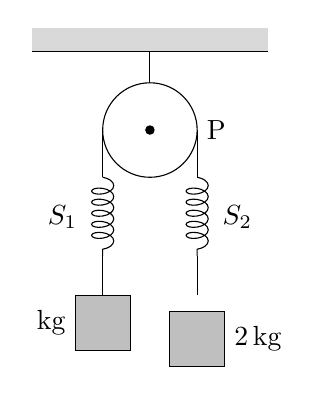
\begin{tikzpicture}
% ceiling
\fill[gray!30] (-1.5,5) rectangle (1.5,5.3);
\draw (-1.5,5) -- (1.5,5);
\draw (0,5) -- (0,4.6);
% pulley
\draw (0,4) circle (0.6);
\filldraw (0,4) circle (1.5pt);
\node[right] at (0.6,4) {P};
% rope over pulley
\draw (-0.6,4) -- (-0.6,3.4);
\draw (0.6,4) -- (0.6,3.4);
% spring S1
\draw[decorate,decoration={coil,segment length=4pt,amplitude=4pt}] (-0.6,3.4) -- (-0.6,2.4);
\node[left] at (-0.8,2.9) {$S_1$};
% spring S2
\draw[decorate,decoration={coil,segment length=4pt,amplitude=4pt}] (0.6,3.4) -- (0.6,2.4);
\node[right] at (0.8,2.9) {$S_2$};
% ropes to masses
\draw (-0.6,2.4) -- (-0.6,1.9);
\draw (0.6,2.4) -- (0.6,1.9);
% masses
\fill[gray!50] (-0.95,1.2) rectangle (-0.25,1.9); \draw (-0.95,1.2) rectangle (-0.25,1.9);
\node[left] at (-0.95,1.55) {kg};
\fill[gray!50] (0.25,1.0) rectangle (0.95,1.7); \draw (0.25,1.0) rectangle (0.95,1.7);
\node[right] at (0.95,1.35) {2\,kg};
\end{tikzpicture}
